\documentclass[../main.tex]{subfiles}
\begin{document}
\chapter{Line, Area, Surface, and Volume Integrals}
\section{Line Integrals}
\subsection{Definitions}
\begin{definition}
  Given a curve $C$ parameterised by $t \in [a, b]$, the \textit{line integral} of a vector field $\vec{F}$ along $C$ is:
  \[
    \int_{C} \vec{F} \cdot \d{\vec{x}} = \int_{a}^{b} \vec{F}(\vec{x}(t)) \cdot \deriv{\vec{x}}{t} \d{t}
  \]
\end{definition}
An alternative, but equivalent definition, is to split the curve up at points $\vec{x}_0, \ldots, \vec{x}_n$ on the curve in that order with $\vec{x}_0 = \vec{x}(a)$ and $\vec{x}_N = \vec{x}(b)$.
We then let $\delta \vec{x}_n = \vec{x}_{n + 1} - \vec{x}_n$ for $n \in \{0, \ldots, N - 1\}$.
Then we define the line integral as:
\[
  \int_{C} \vec{F} \cdot \d{\vec{x}} = \lim_{\Delta \to 0} \sum_{n = 0}^{N-1} \vec{F}(\vec{x}_n) \cdot \delta \vec{x}_n
\]
where $\Delta = \max\limits_{0 \leq n \leq N - 1}|\delta \vec{x}_n|$.
Note that as $\Delta \to 0$, we must have $N \to \infty$ so that we still cover the whole curve.
\begin{remark}
  Less commonly, other types of line integral can also be used.
  For example:
  \[
    \int_{C} f(\vec{x}) \d{s} = \int_{a}^{b} f(\vec{x}(t))\abs{\deriv{\vec{x}}{t}} \d{t}
  \]
  as $\deriv{s}{t} = \abs{\deriv{\vec{x}}{t}}$ from \cref{arcLength}.

  Or:
  \[
    \int_{C} \vec{F} \times \d{\vec{x}} = \int_{a}^{b} \vec{F}(\vec{x}(t)) \times \deriv{\vec{x}}{t} \d{t}
  \]
\end{remark}
\begin{remark}[Dynamics and Relativity]
  We saw in Dynamics and Relativity that if $\vec{F}$ is a force being applied to a particle at $\vec{x}(t)$, then $\int_{C} \vec{F} \cdot \d{\vec{x}}$ is called the \textit{work done} by the force along $C$.
\end{remark}
\begin{definition}[Circulation]
If $C$ is a closed curve, then the line integral around the whole curve is denoted:
\[
  \oint_C \vec{F} \cdot \d{\vec{x}}
\]
which is sometimes known as \textit{circulation} of $\vec{F}$ around $C$.
\end{definition}
\begin{remark}
  It does not matter where we start a line integral over a closed loop, provided that we go all the way around.
\end{remark}
We can reverse line integrals using:
\[
  \int_{-C} \vec{F} \cdot \d{\vec{x}} = - \int_{C} \vec{F} \cdot \d{\vec{x}}
\]
and split them up using:
\[
  \int_{C_1 + C_2} \vec{F} \cdot \d{\vec{x}} = \int_{C_1} \vec{F} \cdot \d{\vec{x}} + \int_{C_2} \vec{F} \cdot \d{\vec{x}}
\]
\subsection{Examples}
\begin{example}[Examples of Line Integrals]
  \label{lineIntegralExamples}
  \begin{enumerate}
    \item Integrate $\vec{F} = (y, -x, 0)$ on the straight line $C_1$ joining $(-1, 0, 0)$ and $(1, 0, 0)$.

      We can parametrise the curve as $\vec{x} = (t, 0, 0)$ for $t \in [-1, 1]$.
      Then:
      \[
        \vec{F}(\vec{x}(t)) = (0, -t, 0) \text{ and } \dot{\vec{x}} = (1, 0, 0)
      \]
      so
      \[
        \int_{C_1} \vec{F} \cdot \d{\vec{x}} = \int_{C_1} \vec{0} \cdot \d{\vec{x}} = 0
      \]
    \item Integrate $\vec{F} = (3x^2, 2y, 0)$ on $C_1$.

      We have:
      \[
        \vec{F} \cdot \dot{\vec{x}} = (3t^2, 0, 0) \cdot (1, 0, 0) = (3t^2, 0, 0)
      \]
      so:
      \[
        \int_{C_1} \vec{F} \cdot \d{\vec{x}} = \int_{-1}^{1} 3t^2 \d{t} = \eval{x^3}{-1}{1} = 2
      \]
    \item Integrate $\vec{F} = (y, -x, 0)$ along the curve $C_2$ joining $(-1, 0, 0)$ to $(1, 0, 0)$ parameterised by $\vec{x} = (t - 1, t(t - 2), t(t^2 - 4))$ for $t \in [0, 2]$.

      We have:
      \[
        \vec{F} = (t(t - 2), 1 - t, 0) \text{ and } \dot{\vec{x}} = (1, 2t - 2, 3t^2 - 4)
      \]
      so:
      \[
        \int_{C_2} \vec{F} \cdot \d{\vec{x}} = \int_{0}^{2} (t(t - 2) - 2(t - 1)^2) \d{t} = \eval{-\frac{1}{3}t^3 + t^2 - 2t}{0}{2} = -\frac{8}{3}
      \]
    \item Integrate $\vec{F} = (3x^2, 2y, 0)$ on $C_2$.

      We have:
      \begin{align*}
        \vec{F} \cdot \dot{\vec{x}} &= (3(t - 1)^2, 2t(t - 2), 0) \cdot (1, 2t - 2, 3t^2 - 4) \\
                                    &= 4t^3 - 9t^2 + 2t + 3
      \end{align*}
      so:
      \[
        \int_{C_2} \vec{F} \cdot \d{\vec{x}} = \int_{0}^{2} 4t^3 - 9t^2 + 2t + 3 \d{t} = \eval{t^4 - 3t^3 + t^2 + 3t}{0}{2} = 2
      \]
    \item What is the work done by a force field $\vec{F} = (y^2 e^{x}, e^{y} + 2ye^{x}, 0)$ moving a particle along $C_3$, which is the ellipse $x^2/a^2 + y^2/b^2 = 1$ in the $x$-$y$ plane starting at $(a, 0, 0)$ and going anticlockwise to $(0, b, 0)$.

      We can parametrise this ellipse as $\vec{x}(\theta) = (a \cos \theta, b \sin \theta, 0)$ for $\theta \in [0, \frac{\pi}{2}]$.
      We then have:
      \[
        \vec{F}(\vec{x}(\theta)) = (b^2 \sin^2 \theta e^{a \cos \theta}, e^{b \sin \theta} + 2b\sin\theta e^{a \cos \theta}, 0)
      \]
      and:
      \[
        \deriv{\vec{x}}{\theta} = (-a \sin \theta, b \cos \theta, 0)
      \]
      so:
      \[
        \vec{F} \cdot \deriv{\vec{x}}{\theta} = -ab^2 \sin^3 \theta e^{a \cos \theta} + b \cos \theta e^{b \sin \theta} + 2b^2 \sin \theta \cos \theta e^{a \cos \theta}
      \]
      We can now evaluate the integral:
      \begin{align*}
        \int_{C_3} \vec{F} \cdot \d{\vec{x}} &= \eval{e^{b \sin \theta}}{0}{\pi/2} + \int_{0}^{\pi/2} b^2 \sin \theta e^{a \cos \theta} (-a + 2\cos \theta + a \cos^2 \theta) \d{\theta} \\
                                             &= e^{b} - 1 + \int_{1}^{0} b^2e^{ai}(1 - 2u - au^2) \d{u} \text{ using $u = \cos \theta$}\\
                                             &= e^{b} - 1 + \eval{b^2 e^{au}(1 - u^2)}{1}{0} \\
                                             &= e^{b} - 1 + b^2
      \end{align*}
      If we instead went around the whole ellipse, starting at $(a, 0, 0)$ and going anticlockwise all the way around, we would find that $\oint \vec{F} \cdot \d{\vec{x}} = 0$.
    \item We can also integrate along a path parameterised in a different coordinate system, for example, cylindrical polar coordinates (\cref{cylindricalPolar}).

      Integrate $\vec{F} = z \vec{e}_\phi$ on the path $C_4$ given by $\rho = z^2$, $\phi = \pi z$ for $z = 0$ to $z = 1$.

      We know from \cref{cylindricalInfinitesimals} that:
      \[
        \d{\vec{x}} = \d{\rho}\vec{e}_\rho + \rho \d{\phi}\vec{e}_\phi + \d{z}\vec{e}_z
      \]
      so:
      \[
        \d{\vec{x}} = (2z\vec{e}_\rho + \pi \rho \vec{e}_\phi + \vec{e}_z) \d{z}
      \]
      as $\deriv{\rho}{z} = 2z$ and $\deriv{\phi}{z} = \pi$.
      We then have $\vec{F} \cdot \d{\vec{x}} = \pi \rho z \d{z} = \pi z^3 \d{z}$ and so:
      \[
        \int_{C_4} \vec{F} \cdot \d{\vec{x}} = \int_{0}^{1} \pi z^3 \d{z} = \frac{\pi}{4}
      \]
  \end{enumerate}
\end{example}
\subsection{Path Independence}
\begin{definition}[Exact Differential]
  We say that the differential form $\vec{F} \cdot \d{\vec{x}}$ is \textit{exact} if there exists a single valued scalar field $f(\vec{x})$ such that:
  \[
    \vec{F} \cdot \d{\vec{x}} = F_i \d{x_i} = \d{f}
  \]
  for all $\d{\vec{x}}$.
\end{definition}
\begin{remark}[Recap]
  We saw exact differentials in 2D in IA Differential Equations.
\end{remark}
We also know from \cref{infinitesimalsGrad} that $\d{f} = \nabla f \cdot \d{\vec{x}}$ and so $\vec{F} \cdot \d{\vec{x}}$ is exact if and only if there exists a single valued function such that $\vec{F} = \nabla f$, that is, it is exact if and only if $\vec{F}$ is a conservative (\cref{conservativeField}) field.

\begin{proposition}
  If $\vec{F} = \nabla f$ is a conservative vector field and $C$ is a path from $a$ to $b$, then:
  \[
    \int_{C} \vec{F} \cdot \d{\vec{x}} = f(\vec{b}) - f(\vec{a})
  \]
  So the line integral depends only on the endpoints of the path.
\end{proposition}
\begin{proof}
  We can write $\vec{F} = \nabla f$ and so $\d{f} = \nabla f \cdot \d{\vec{x}} = \vec{F} \cdot \d{\vec{x}}$.
  Substituting this into the integral:
  \[
    \int_{C} \vec{F} \cdot \d{\vec{x}} = \int_{C} \d{f} = \eval{f}{\vec{a}}{\vec{b}} = f(\vec{b}) - f(\vec{a})
  \]
\end{proof}
\begin{proof}[Alternative]
Since $\deriv{f}{t} = \dot{\vec{x}} \cdot \nabla f$ from \cref{MVCGrad}, we have:
\[
  \int_{C} \vec{F} \cdot \d{\vec{x}} = \int_{C} \nabla f \cdot \dot{\vec{x}} \d{t} = \int \deriv{f}{t} \d{t} = f(\vec{b}) - f(\vec{a})
\]
\end{proof}
\begin{remark}[Notation]
  Since the value of the line integral is independent of the particular path $C$ between $\vec{a}$ and $\vec{b}$, we can write  $\int_{\vec{a}}^{\vec{b}} \vec{F} \cdot \d{\vec{x}}$ without ambiguity.
  We usually would not be able to do this as different paths would result in different values, hence why we usually specific a path $C$.
\end{remark}
\begin{corollary}
  If $\vec{F}$ is conservative and $C$ is a closed curve, then $\oint_C \vec{F} \cdot \d{\vec{x}} = 0$.
\end{corollary}
\begin{proof}
  Since $\vec{F}$ is conservative, we can write $F = \nabla f$ for a \textbf{single valued} $f$.
  The curve is closed so the value of the integral is $f(\vec{a}) - f(\vec{a})$ which is zero since $f$ is single valued.
\end{proof}
\begin{proposition}
  In a \textbf{simply connected domain}, the following are equivalent:
  \begin{enumerate}
    \item $\vec{F}$ is a conservative vector field.
    \item There exists a single valued $f(\vec{x})$ such that $\vec{F} = \nabla f$.
    \item $\vec{F} \cdot \d{\vec{x}}$ is an exact differential.
    \item $\vec{F}$ is irrotational.
    \item $\nabla \times \vec{F} = \vec{0}$.
    \item $\pderiv{F_i}{x_j} = \pderiv{F_j}{x_i}$ for all $i, j$
    \item For any $\vec{a}, \vec{b}$ in the domain of $\vec{F}$, $\int_{\vec{a}}^{\vec{b}} \vec{F} \cdot \d{\vec{x}}$ is path independent.
    \item $\oint_C \vec{F} \cdot \d{\vec{x}} = 0$ for all closed curves $C$ in the domain.
  \end{enumerate}
\end{proposition}
\begin{proof}
  \begin{itemize}
    \item \textbf{i} $\iff$ \textbf{ii} and \textbf{iv} $\iff$ \textbf{v} by definition.
    \item \textbf{i} $\iff$ \textbf{iii} was shown above.
    \item \textbf{i} $\iff$ \textbf{iv}, see \cref{conservativeFields}.
    \item \textbf{v} $\iff$ \textbf{vi} by considering components of $\nabla \times \vec{F}$:
      \[
        [\nabla \times \vec{F}]_k = \levi_{i j k} \pderiv{F_j}{x_i} = 0
      \]
      which is true for all $k$ if and only if $\pderiv{F_j}{x_i}$ is symmetric in $i$ and $j$.
    \item \textbf{ii} $\implies$ \textbf{vii} was shown above.
    \item \textbf{vii} $\implies$ \textbf{viii}, given any closed curve $C$ we can split it into two parts, $C_1$ from $\vec{a}$ to $\vec{b}$, then $C_2$ from $\vec{b}$ back to $\vec{a}$ so that $C = C_1 + C_2$, but, by assumption, since $C_1$ and $-C_2$ have the same endpoints:
      \[
        \int_{C_1} \vec{F} \cdot \d{\vec{x}} = \int_{-C_2} \vec{F} \cdot \d{\vec{x}} = - \int_{C_2} \vec{F} \cdot \d{\vec{x}}
      \]
      and so:
      \[
        \oint_C \vec{F} \cdot \d{\vec{x}} = \int_{C_1} \vec{F} \cdot \d{\vec{x}} + \int_{C_2} \vec{F} \cdot \d{\vec{x}} = 0
      \]
  \end{itemize}
  This leaves \textbf{viii} $\implies$ \textbf{vii} and \textbf{vii} $\implies$ \textbf{ii} which will be proved in the next chapter.
\end{proof}
\begin{example}[Revisiting \cref{lineIntegralExamples}]
  \begin{itemize}
    \item In \textbf{i} and \textbf{iii}, we integrated $\vec{F} = (y, -x, 0)$ along two different paths.
      We see that $\vec{F}$ is not conservative as $\nabla \times \vec{F} = (0, 0, -2) \neq \vec{0}$.
      This agrees with how we got two different values for the line integral on the two different paths, despite the fact that they had the same end points.
    \item In \textbf{ii} and \textbf{iv} we integrated $\vec{F} = (3x^2, 2y, 0)$ along two different paths.
      Here $\vec{F}$ is conservative as $\nabla \times \vec{F} = \vec{0}$.
      We can also just spot that $\vec{F} = \nabla (x^3 + y^2)$, and so it follows that $\vec{F}$ is conservative as it has a single valued scalar potential.

      Therefore the value of the integral is path independent so:
      \[
        \int_{(-1, 0, 0)}^{(1, 0, 0)} \vec{F} \cdot \d{\vec{x}} = \eval{x^3 + y^2}{(-1, 0, 0)}{(1, 0, 0)} = 2
      \]
      which agrees with our answers, despite the different paths.
    \item In \textbf{v}, we integrated $\vec{F} = (y^2 e^{x}, e^{y} + 2ye^{x}) = \nabla(e^{y}, y^2e^{x})$ which is conservative and so we can shortcut the rather involved integration to obtain:
      \[
        \int_{C_3} \vec{F} \cdot \d{\vec{x}} = \eval{e^{y} + y^2e^{x}}{(a, 0, 0)}{(0, b, 0)} = e^{b} + b^2 - 1
      \]
      which agrees with our answer.
    \item In \textbf{vi}, we integrated $F = z \vec{e}_\phi$.
      Using \cref{cylindricalOperators}, we see that $\nabla \times (z \vec{e}_\phi) = -\vec{e}_\rho \neq \vec{0}$ and so $\vec{F}$ is not conservative.

      Suppose that $\nabla \times \vec{F}$ had actually been $\vec{0}$, we could not have concluded that $\vec{F}$ would be conservative.
      The domain of $\vec{F}$ does not include the $z$-axis apart from $\vec{0}$ as $\vec{e}_\phi$ is not defined there.
      So we could shrink a curve around the $z$ axis to a point by passing it through the ``gap'' at the origin, however, the derivatives of $F$ are not defined at the origin and so $\nabla \times \vec{F}$ is also not defined there so we are not working in a simply connected domain.
  \end{itemize}
\end{example}
\section{Area Integrals}
\subsection{Definition}
To integrate over a region $A \subset \R^2$, we cover $A$ with a large number $N$ of small disjoint subsets $\delta A_i \subset A$ for $i \in \{1, \ldots, N\}$.
Then:
\[
  \int_A f(x, y) \d{x} = \lim_{\Delta \to 0} \sum_{i = 1}^{N} f(x_i, y_i) \delta A_i
\]
where $(x_i, y_i) \in \delta A_i$ and $\Delta$ is the maximum linear dimension of all the $\delta A_i$, and as $\Delta \to 0$, $N \to \infty$ so that the shrinking subsets still cover the entirety of $A$.

Informally, we can think of $\int_A f(x, y) \d{A}$ is the volume under the graph of $z = f(x, y)$, similarly to how we can think of $\int_{a}^{b} f(x) \d{x}$ as the area under the graph $y = f(x)$.
\begin{remark}[Note]
  $A$ refers to both the region itself and its area so:
  \[
    A = \int_A 1 \d{A}
  \]
\end{remark}
\begin{remark}
  It does not matter how we divide $A$ up, every different way will lead to the same answer as $\Delta \to 0$.

  If it doesn't give the same answer, then we say that $f$ is not integrable of $A$ but for most reasonable functions $f$ and regions $A$, it will be integrable.
\end{remark}
The most obvious way to divide $A$ up is to use rectangles parallel to the $x$ and $y$ axes with area $\delta x \delta y$.

If we first sum over a horizontal strip of $y$ with constant height $\delta y$ and let $\delta x \to 0$ then we obtain:
\[
  \left(\int_{X(y)} f(x, y) \d{x}\right)\delta y
\]
where for each $y$, $X(y) = \{x: (x, y) \in A\}$.
We then sum these over the range of $y$ and let $\delta y \to 0$ to obtain:
\[
  \int_{y_{\text{min}}}^{y_{\text{max}}} \left(\int_{X(y)} f(x, y) \d{x}\right) \d{y}
\]

We could also sum vertical strips to obtain:
\[
  \int_{x_{\text{min}}}^{x^{\text{max}}} \left(\int_{Y(x)} f(x, y) \d{y}\right) \d{x}
\]
where $Y(x) = \{y: (x, y) \in A\}$.

\textit{Fubini's Theorem} tells us that both of these are equal to $\int_A f(x, y) \d{A}$ for any reasonable $f$ and $A$.
That is, taking the limits in $x$ and then $y$, is the same as taking the limits in $y$ and then $x$, and the same as taking $\Delta \to 0$.
\begin{remark}[Restrictions on Fubini's Theorem]
  \nonexaminable
  When we mean reasonable $f$ and $A$, the restrictions are quite loose, if $f$ is piecewise continuous and the boundary of $A$ is a finite piecewise smooth curve then Fubini's Theorem holds.
\end{remark}
\begin{remark}[Notation]
  Some other notation for $\int_A f(x, y) \d{A}$  include:
  \[
    \int_A f(x, y) \d{x} \d{y},\ \int_A f(\vec{x}) \d^2{\vec{x}},\ \iint\limits_A f(x, y) \d{A},\ \int_A f(x, y) \d{S},\ \int\d{x}\int\d{y} f(x, y)
  \]
\end{remark}
\begin{example}
  Integrate $f(x, y) = xy^2$ over $A$, a triangle with vertices at $(0, 0), (1, 1)$ and $(1, -1)$.

  \begin{center}
  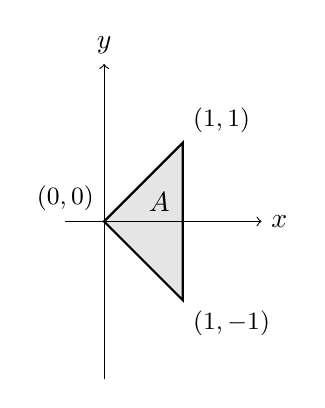
\begin{tikzpicture}
    \filldraw[fill=gray!20, draw=black, thick] (0, 0) node[above left] {\small$(0, 0)$} -- (1, 1) node[above right] {\small$(1, 1)$} -- (1, -1) node[below right] {\small$(1, -1)$} -- cycle;
    \node[above] at (0.7, 0) {$A$};
    \draw[->] (-0.5, 0) -- (2, 0) node[right] {$x$};
    \draw[->] (0, -2) -- (0, 2) node[above] {$y$};
  \end{tikzpicture}
  \end{center}

  We can integrate over $y$ first:
  \begin{align*}
    \int_A f(x, y) \d{A} &= \int_{0}^{1} \int_{-x}^{x} xy^2 \d{y} \d{x} \\
                         &= \int_{0}^{1} x \eval{\frac{1}{3} y^3}{-x}{x} \d{x} \\
                         &= \int_{0}^{1} \frac{2}{3}x^{4} \d{x} \\
                         &= \frac{2}{15}
  \end{align*}
  We can also integrate over $x$ first, although the bounds are a bit more fiddly:
  \begin{align*}
    \int_A f(x, y) \d{A} &= \int_{-1}^{1} \int_{|y|}^{1} xy^2 \d{x} \d{y} \\
                         &= \int_{-1}^{1} y^2 \eval{\frac{1}{2}x^2}{|y|}{1} \d{y} \\
                         &= \int_{-1}^{1} \frac{1}{2}y^2(1 - y^2) \d{y} \\
                         &= \frac{1}{3} - \frac{1}{5} = \frac{2}{15}
  \end{align*}
\end{example}
\begin{remark}[Warning]
  Make sure that you determine the inner limits in terms of the outer variable.
  A common mistake is to just make both limits run between the min and max of $x$ and $y$, however, this means that you will always be integrating over a rectangle.
\end{remark}
\begin{remark}[Special Case]
  If $A$ is a rectangle, i.e. $A = \{(x, y): x \in [a, b], y \in [c, d]\}$, and $f$ is \textit{separable} so it can be written as $f(x, y) = g(x)h(y)$, then we can do the $x$-integral first, pulling out $h(y)$:
  \[
    \int_{X(y)} f(x, y) \d{x} = h(y) \int_{a}^{b} g(x) \d{x}
  \]
  Now when we do the outer integral, $\int_{a}^{b} g(x) \d{x}$ is just a constant so can be pulled out so:
  \[
    \int_A f(x, y) \d{A} = \left(\int_{a}^{b} g(x) \d{x}\right)\left(\int_{c}^{d} h(y) \d{y}\right)
  \]
\end{remark}
\subsection{Change of Variables}
\begin{proposition}[Change of variables for area integrals]
  If $(u, v) \mapsto (x, y)$ is a bijection from a region $A'$ in the $(u, v)$-plane to the region $A$ in the $(x, y)$-plane, then:
  \[
    \int_A f(x, y) \d{x} \d{y} = \int_{A'} F(u, v) \abs{\frac{\partial(x, y)}{\partial(u, v)}} \d{u}\d{v}
  \]
  where $F(u, v) = f(x(u, v), y(u, v))$ and:
  \[
    J = \frac{\partial(x, y)}{\partial(u, v)} \equiv \det \begin{pmatrix}
    \pderiv{x}{u} & \pderiv{x}{v} \\
    \pderiv{y}{u} & \pderiv{y}{v} \\
    \end{pmatrix}
  \]
  is called the \textit{Jacobian} of the transformation.
\end{proposition}
\begin{remark}[Note]
  It is the \textbf{modulus} of $J = \frac{\partial(x, y)}{\partial(u, v)}$ that appears in this rule, not a determinant.
  That is, we have a factor of $|J|$ where $J$ is the \textbf{determinant} of a matrix.
\end{remark}
\begin{remark}[Notation]
  We often just call $F$ just $f$ so the right hand side reads:
  \[
    \int_{A'} f(u, v) |J| \d{u} \d{v}
  \]
  which is clearly incorrect but regardless it is usually clear what is meant.
\end{remark}
\begin{proof}
  We can choose how we want to divide $A$ up and so we choose to divide $A$ up into small regions between curves of constant $u$ and constant $v$.
  In \cref{surfaceElements}, we saw how we can find the area of such a region on a 2D surface, so, as we can consider $A$ a flat surface in the $(x, y)$-plane, the area of each region is given by:
  \[
    \abs{\pderiv{\vec{x}}{u} \times \pderiv{\vec{x}}{v}} \d{u} \d{v} = \abs{\begin{pmatrix}
    \pderiv{x}{u} \\
    \pderiv{y}{u} \\
    0 \\
    \end{pmatrix} \times \begin{pmatrix}
    \pderiv{x}{v} \\
    \pderiv{y}{v} \\
    0 \\
    \end{pmatrix}} \d{u} \d{v} =
    \abs{\pderiv{x}{u}\pderiv{y}{v} - \pderiv{x}{v}\pderiv{y}{u}}\d{u}\d{v} = |J| \d{u}\d{v}
  \]
  The contribution of this particular region to the sum defining $\int_A f \d{A}$ is therefore $f(\vec{x}(u, v))|J| \d{u} \d{v} = F(u, v) |J| \d{u} \d{v}$.
  Integrating over the values of $(u, v) \in A'$, we have:
  \[
    \int_A f \d{x} \d{y} = \int_{A'} F |J|\d{u} \d{v}
  \]
\end{proof}
\begin{remark}
  The goal of using such a transform is either to simplify the region of integration and/or the integrand.
\end{remark}
\begin{example}
  Evaluate the integral $\int_A y^2 \d{A}$ where $A$ is the semicircular domain $\{(x, y): x^2 + y^2 < R^2,\ y > 0\}$.

  We choose plane polar coordinates $(r, \theta)$ defined by $x = r\cos \theta$, $y = r\sin\theta$.
  Then in the $(r, \theta)$-plane, we see that there is a bijection between the rectangle $A' = \{(r, \theta): r < R,\ 0 < \theta < \pi\}$ and $A$.

  We first find the Jacobian of the transformation:
  \[
    |J| = \det \begin{pmatrix}
    \pderiv{x}{r} & \pderiv{x}{\theta} \\
    \pderiv{y}{r} & \pderiv{y}{\theta} \\
    \end{pmatrix} = \det \begin{pmatrix}
    \cos \theta & -r\sin \theta \\
    \sin \theta & r\cos \theta \\
    \end{pmatrix} = r
  \]
  We also find that $F(r, \theta) = f(r \cos \theta, r \sin \theta) = r^2 \sin^2 \theta$ and so:
  \[
    \int_A y^2 \d{A} = \int_{A'} r^2 \sin^2 \theta |r| \d{r} \d{\theta}
  \]
  Since $F$ separable and we are integrating over the rectangle $A'$, we obtain:
  \[
    \int_{0}^{R} r^3 \d{r} \int_{0}^{\pi} \sin^2\theta \d{\theta} = \frac{1}{8}\pi R^4
  \]

  In this example, the area element was $\d{A'} = r \d{r} \d{\theta}$:
  \begin{center}
  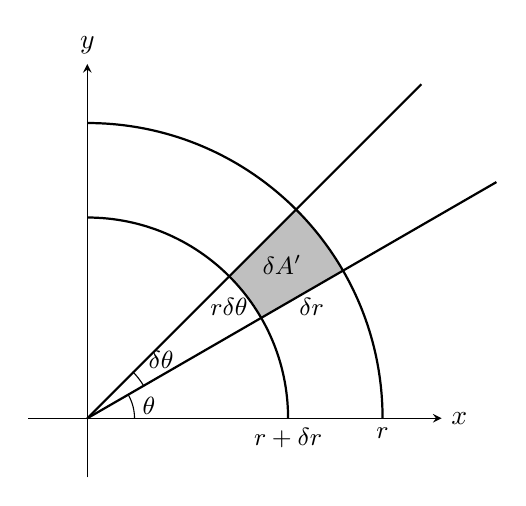
\begin{tikzpicture}[>=stealth, scale=1.5]
    \begin{scope}
      \clip (0, 0) -- (3, 3) -- (2.165, 1.25);
      \fill[gray!50] (0, 0) circle (2.5);
      \fill[white] (0, 0) circle (1.7);
    \end{scope}
    \begin{scope}
      \clip (0, 0) rectangle (3, 3);
      \draw[thick] (0, 0) circle (2.5);
      \draw[thick] (0, 0) circle (1.7);
    \end{scope}
    \draw[->] (-0.5, 0) -- (3, 0) node[right] {$x$};
    \draw[->] (0, -0.5) -- (0, 3) node[above] {$y$};
    \draw[rotate = 45, thick] (0, 0) -- (4, 0);
    \draw[rotate = 30, thick] (0, 0) -- (4, 0);
    \node[below] at (2.5, 0) {\small$r$};
    \node[below] at (1.7, 0) {\small$r + \delta r$};
    \node[below] at (1.9, 1.1) {\small$\delta r$};
    \node[below] at (1.2, 1.1) {\small$r \delta \theta$};
    \node at (1.65, 1.3) {\small$\delta A'$};

    \draw (0.4, 0) arc [start angle=0,end angle=30,radius=0.4] node[midway, right] {\small$\theta$};
    \draw (0.48, 0.27) arc [start angle=30,end angle=45,radius=0.6] node[midway, above right] {\small$\delta\theta$};
  \end{tikzpicture}
  \end{center}
  As $\delta r$ and $\delta \theta$ become infinitesimal, the region $\delta A'$ becomes a rectangle and so $\d{A} = (r \d{\theta}) \d{r}$.
\end{example}
\subsection{Properties of the Jacobian}
Let $J_1$ be the Jacobian for $(u, v) \mapsto (x, y)$ and $J_2$ for $(\xi, \eta) \mapsto (u, v)$.
Consider the matrix product:
\begin{align*}
  J_1 J_2 &= \begin{pmatrix}
  \pderiv{x}{u} & \pderiv{x}{v} \\
  \pderiv{y}{u} & \pderiv{y}{v} \\
  \end{pmatrix}
  \begin{pmatrix}
  \pderiv{u}{\xi} & \pderiv{u}{\eta} \\
  \pderiv{v}{\xi} & \pderiv{v}{\eta} \\
  \end{pmatrix} \\
  &= \begin{pmatrix}
  \pderiv{x}{u} \pderiv{u}{\xi} + \pderiv{x}{v} \pderiv{v}{\xi} & \pderiv{x}{u} \pderiv{u}{\eta} + \pderiv{x}{v} \pderiv{v}{\eta} \\
  \pderiv{y}{u} \pderiv{u}{\xi} + \pderiv{x}{v} \pderiv{y}{\xi} & \pderiv{y}{u} \pderiv{u}{\eta} + \pderiv{y}{v} \pderiv{v}{\eta} \\
  \end{pmatrix} \\
  &= \begin{pmatrix}
  \pderiv{x}{\xi} & \pderiv{x}{\eta} \\
  \pderiv{y}{\xi} & \pderiv{y}{\eta} \\
  \end{pmatrix}
\end{align*}
Since $\det(J_1 J_2) = \det(J_1)\det(J_2)$, we see that:
\[
  \frac{\partial(x, v)}{\partial(u, v)} \frac{\partial(u, v)}{\partial(\xi, \eta)} = \frac{\partial(x, y)}{\partial(\xi, \eta)}
\]
So the Jacobian of a composition of maps is the product of the Jacobians.
\end{document}
